\subsection{Diffusion and Fick's Law}
\label{det_diff}
The term diffusion describes the phenomenon that matter migrates in the direction of the negative concentration gradient. In consequence, inhomogeneities in the system tend to spread over time and gradients disappear (cite Atkins, pg.\ 770). Diffusion is an integral part of the Gray-Scott model since it is essential for the pattern formation mechanism. In the following, a deterministic description for diffusion (Fick's law) will be derived to incorporate the phenomenon into the reaction rate equations \eqref{eq:ode1} and \eqref{eq:ode2} given above. 

Let there be a cubic tube filled with a solution of some species A. The tube stretches along the $x$-Axis. The extent in the two other directions is negligibly small and so are possible concentration inhomogeneities in this plane. On the left end, the concentration $a = [A]$ is high, on the right end it is low. Figure \eqref{fig:fickslaw} illustrates the setup. Considering a slab of length $l$ ranging from $x_s$ to $x_s + l$ perpendicular to the $x$-Axis, the change of concentration inside the slab in some infinitesimal time interval is equal to the influx through the cross-sectional area $A$ at $x = x_s$ minus the flux out of the slab at $x = x_s + l$:
\begin{align}
\label{eq:diff_flux}
\frac{\partial a}{\partial t} = \frac{J(x_s) A dt}{A l dt} - \frac{J(x_s + l) A dt}{A l dt} = \frac{J - J'}{l}
\end{align}
The flux $J(x)$ at position $x$ is proportional to the negative concentration gradient $\frac{\partial a}{\partial x}$ at $x$. Using this relation gives 
\begin{align}
\begin{split}
J - J' &= -D \frac{\partial a}{\partial x} + D \frac{\partial a'}{\partial x} \\
&= -D \frac{\partial a}{\partial x} + D \frac{\partial}{\partial x} \left\{ a + \frac{\partial a}{\partial x} l \right\} 
= D l \frac{\partial^2 a}{\partial x^2}
\end{split}
\end{align}
with positive diffusion constant $D$. 

\begin{figure}
\centering
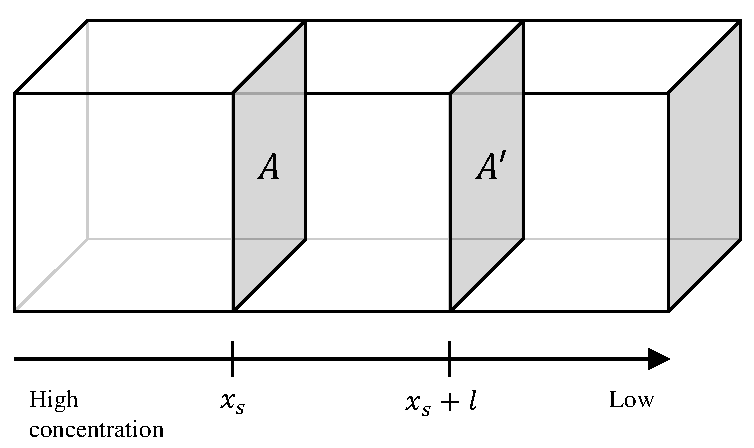
\includegraphics[width=\textwidth]{images/fickslaw.pdf}
\caption{Illustration of the setup used to derive Fick's law of diffusion}
\label{fig:fickslaw}
\end{figure}

By substituting this relation back into \eqref{eq:diff_flux} and by passing the limit $l \to 0$, one obtains the one-dimensional version of Fick's law of diffusion:
\begin{align}
\frac{\partial a}{\partial x} = D \frac{\partial^2 a}{\partial x^2}
\end{align}
In the generalized 3D case, the spatial derivative term turns into the Laplace operator $\Delta u = \frac{\partial^2 u}{\partial x^2} + \frac{\partial^2 u}{\partial y^2} + \frac{\partial^2 u}{\partial z^2}$: 
\begin{align}
\frac{\partial a}{\partial t} = D \Delta u
\end{align}

The complete Gray-Scott model is then discribed by the following partial differential equations:
\begin{gather}
\frac{\partial u}{\partial t} = D_u \Delta u - \rho u v^2 + F(1-u) \\
\frac{\partial v}{\partial t} = D_v \Delta v + \rho u v^2 - (F+\kappa) v
\end{gather}
where $D_u$ and $D_v$ are positive diffusion constants of the species U and V, respectively.